\section{Results}\label{Sec:Results}

\subsection{Descriptive analysis of empirical confidence regions}

The regions used as a reference in this work are obtained through true random sequences, where we extract the empirical distribution of white noises in the Entropy-Complexity plane.
In Fig.~\ref{fig:HC-PCA} we show the results obtained for $T = 50000$ in the scenarios of $D = 3$ and $D = 6$ in the new space defined by the PCA, together with the quantiles of $\SI{90}{\percent}$, $\SI{95}{\percent}$, $\SI{99}{\percent}$, and $\SI{99.9}{\percent}$.
We also show the projection of the $H \times C$ plane limits in this new representation space, as well as identifying the median of each data set, the latter being represented as the red dots present in the graphs.

\begin{figure}
	\centering
	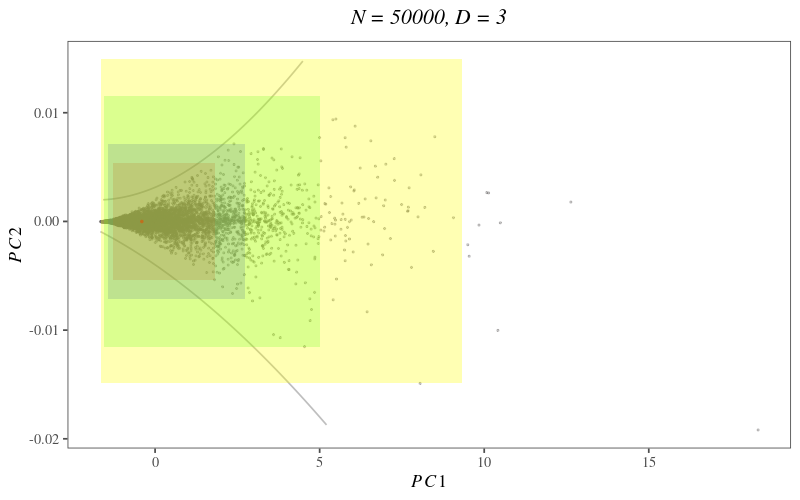
\includegraphics[width=.45\linewidth]{Figures/HC-PCA-Trozos-D3N50k.png}
	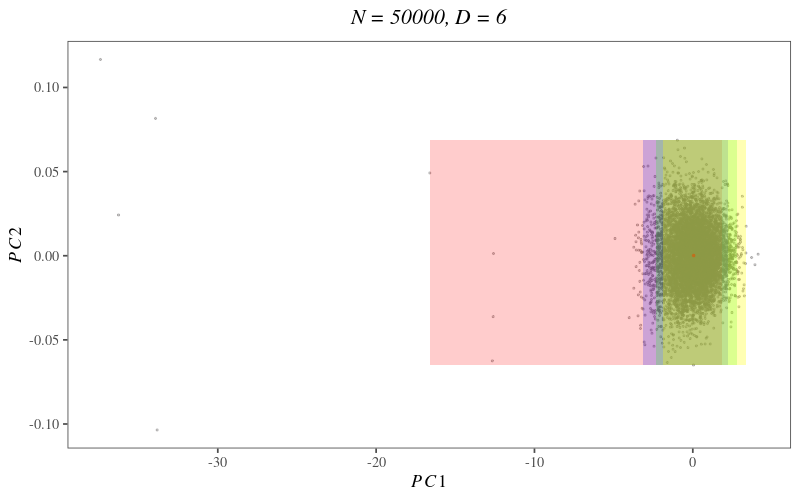
\includegraphics[width=.45\linewidth]{Figures/HC-PCA-Trozos-D6N50k.png}
	\caption{Representation of truly random sequences with length $T = 50.000$ in the PCA space for $D = 3$ and $D = 6$, and the quantiles of $\SI{90}{\percent}$, $\SI{95}{\percent}$, $\SI{99}{\percent}$, and $\SI{99.9}{\percent}$.}
	\label{fig:HC-PCA}
\end{figure} 

As we can see in Fig.~\ref{fig:PCA-Hist} in the new representation space produced by the PCA, the data are not evenly distributed among the axes of the first main component, maintaining the character presented in the $H \times C$ plane, since such points tend to be concentrated close to the point $(1, 0)$.

\begin{figure}
    \centering
    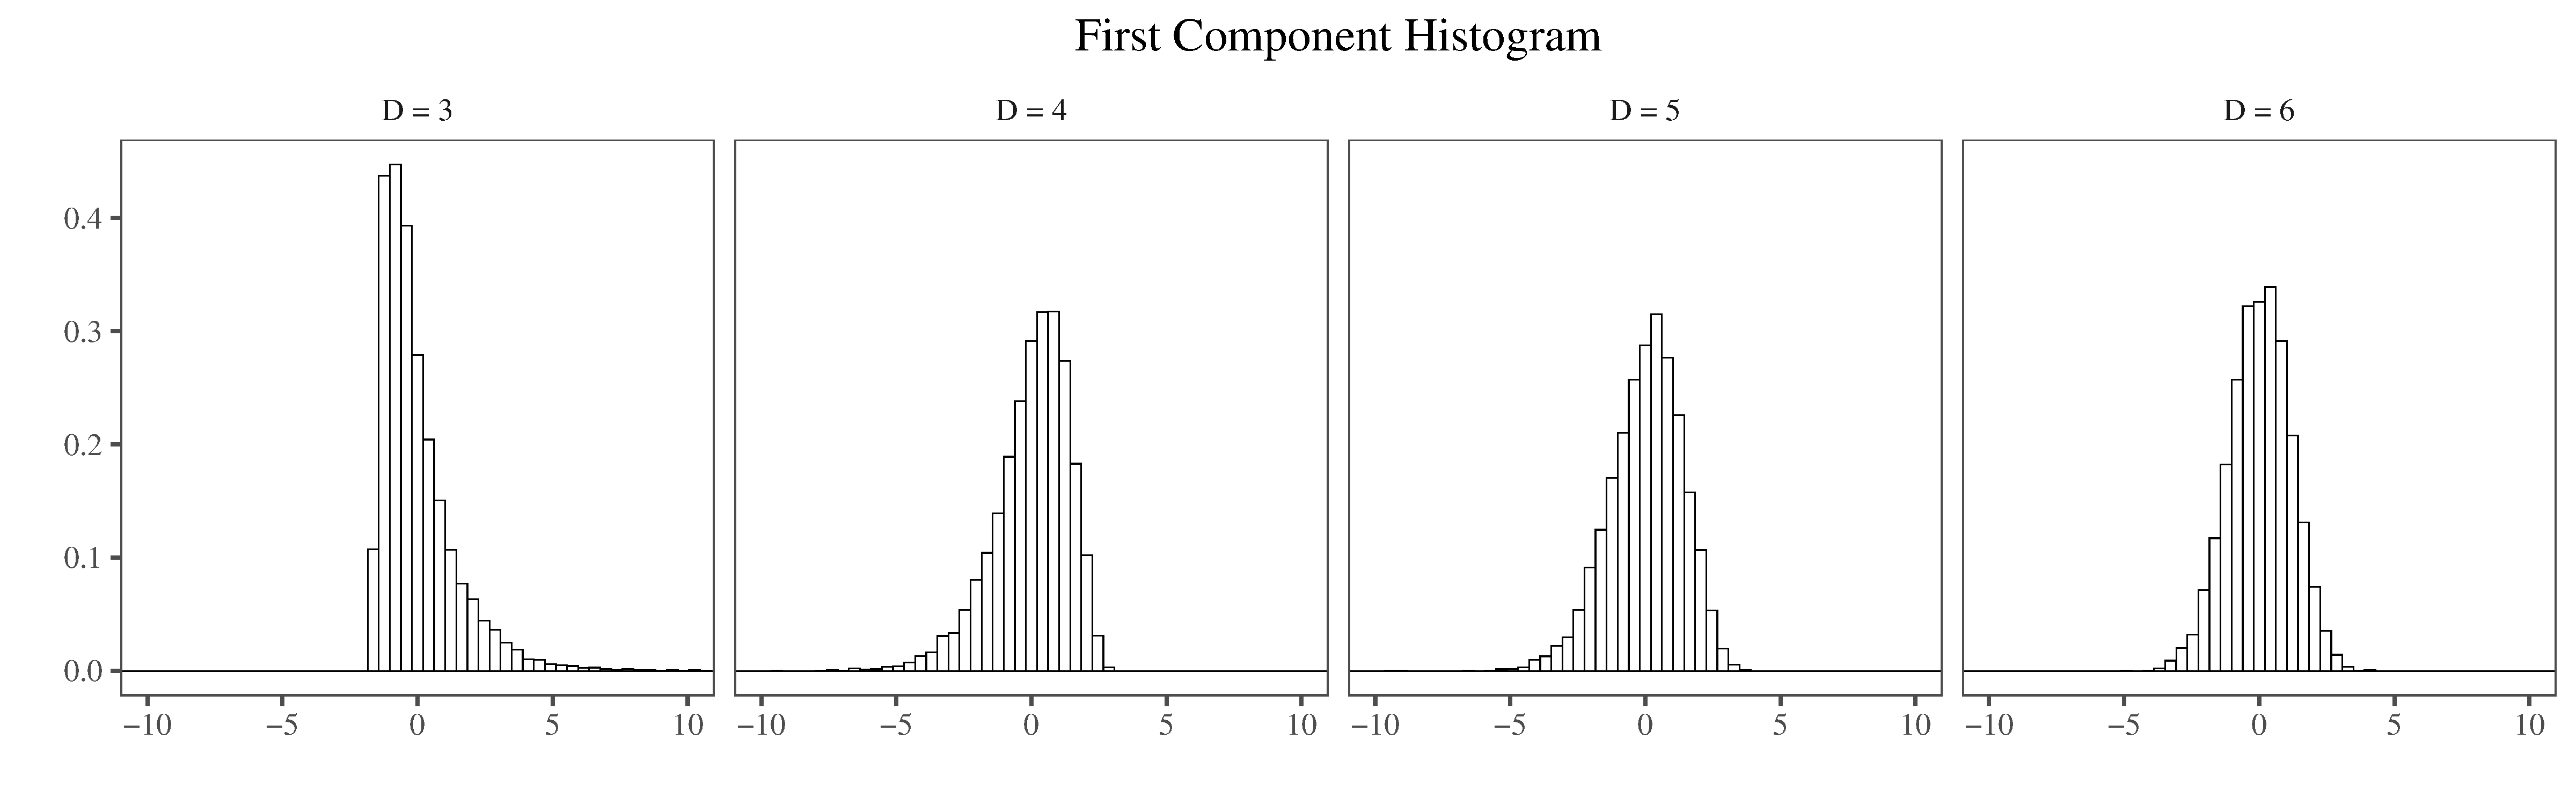
\includegraphics[width=\linewidth]{PCA-hist-50k}
    \caption{Histogram of the PCA first component }
    \label{fig:PCA-Hist}
\end{figure}

\subsection{Testing White Noise in the confidence regions}

To analyze the efficiency of the confidence region calculated, we tested its applicability on a set of true random data generated physically not used by the algorithm during its construction. 
The results can be seen in Fig.~\ref{fig:RNG}.

For small series, $T = 1000$, and $D = 3$ we managed to maintain exactly $\SI{99}{\percent}$ of the data in the confidence region of the same value, and as the dimension increased reach $\SI{96}{\percent}$ of the points.
On the other hand, there was a very large loss of points located in the region with $\SI{95}{\percent}$ confidence as the dimension increased.
A reasonable explanation for this event is given in the choice of the parameter itself.
It is known by definition that $D! << N$, which does not happen for such a sample size, thus presenting many missing patterns that lead to an unrepresentative probability distribution.
For larger series, $T = 50000$, although we observed a small drop in the percentage of data present in the region with $\SI{99}{\percent}$ confidence, there was a significant increase in points in the region with $\SI{95}{\percent}$ confidence, showing between $\SI{90}{\percent}$ and $\SI{88}{\percent}$ of the points when we vary the embedding dimension.

\begin{figure}
    \centering
    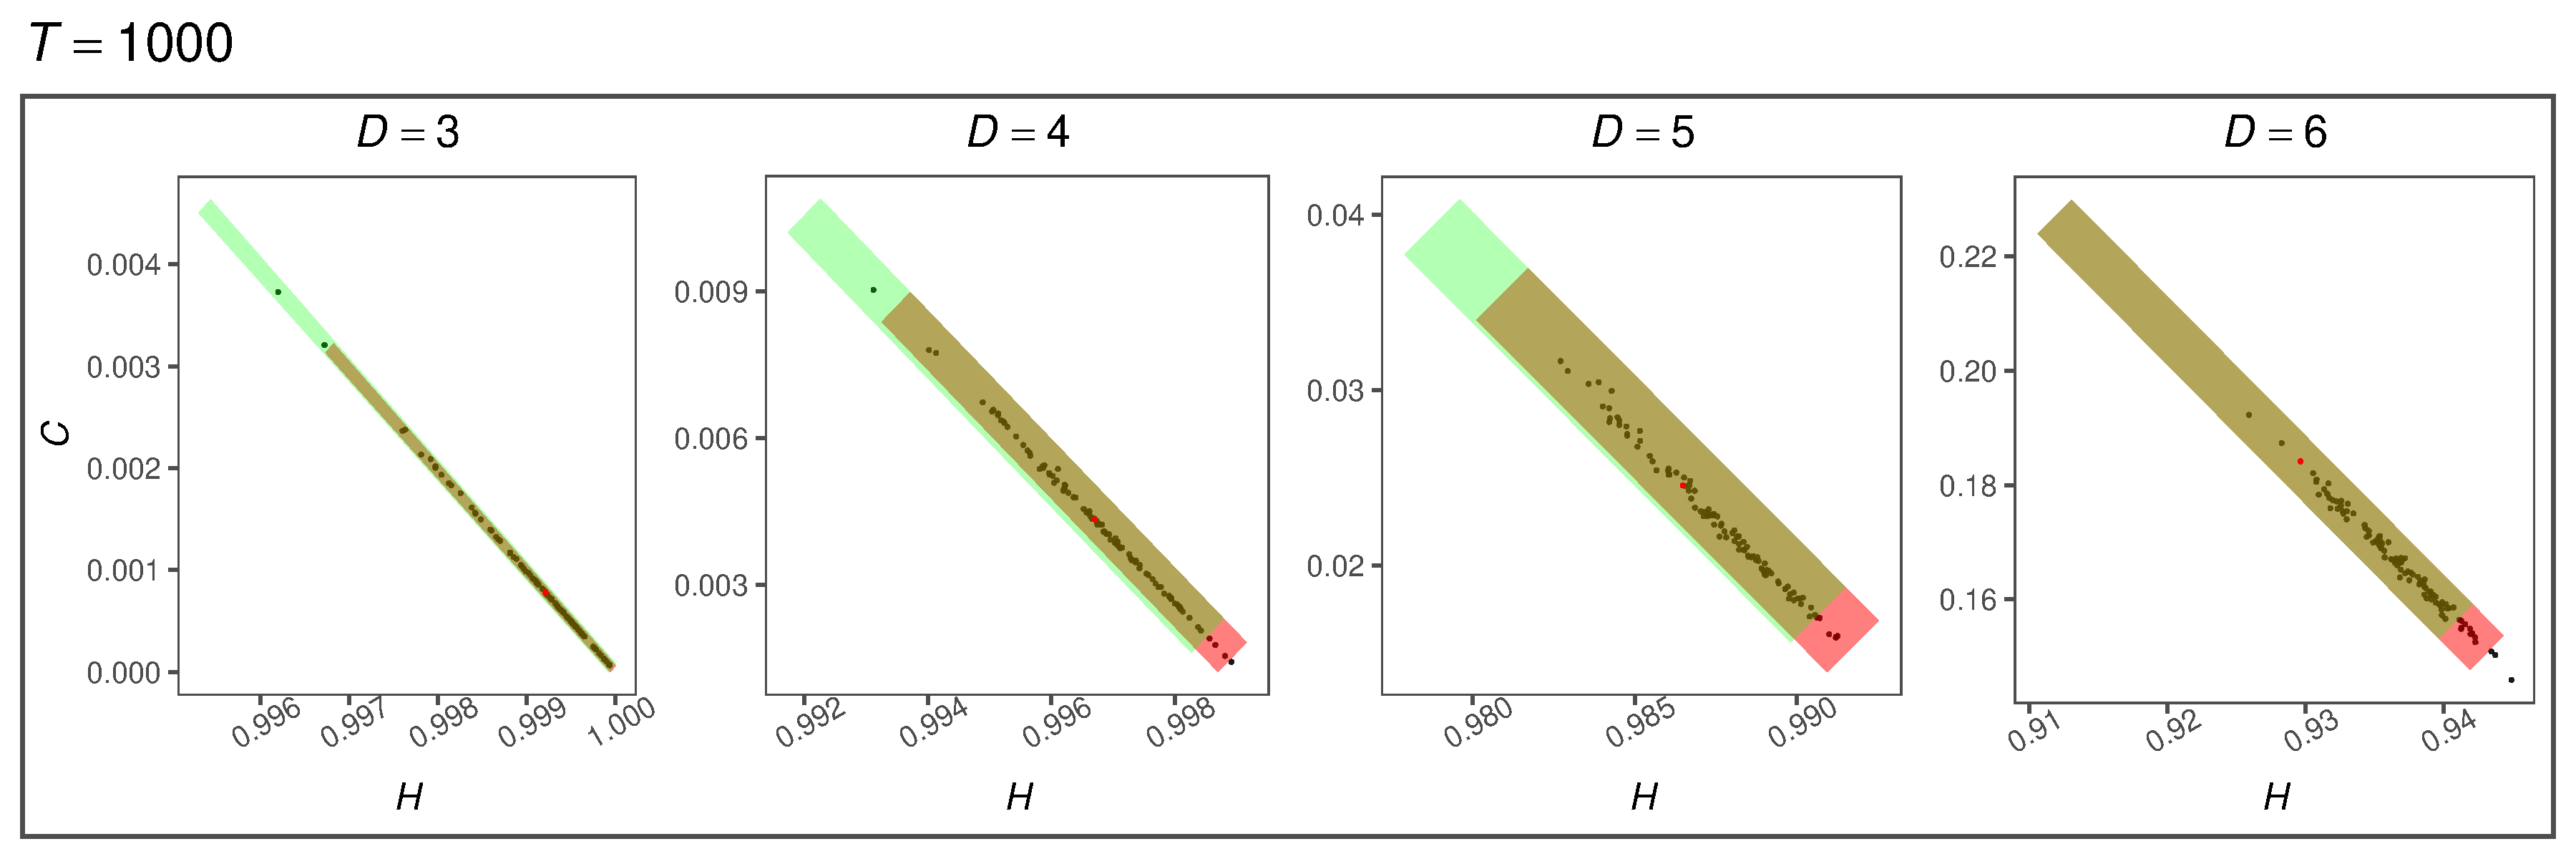
\includegraphics[width=\linewidth]{Figures/RNG-1000.pdf}
    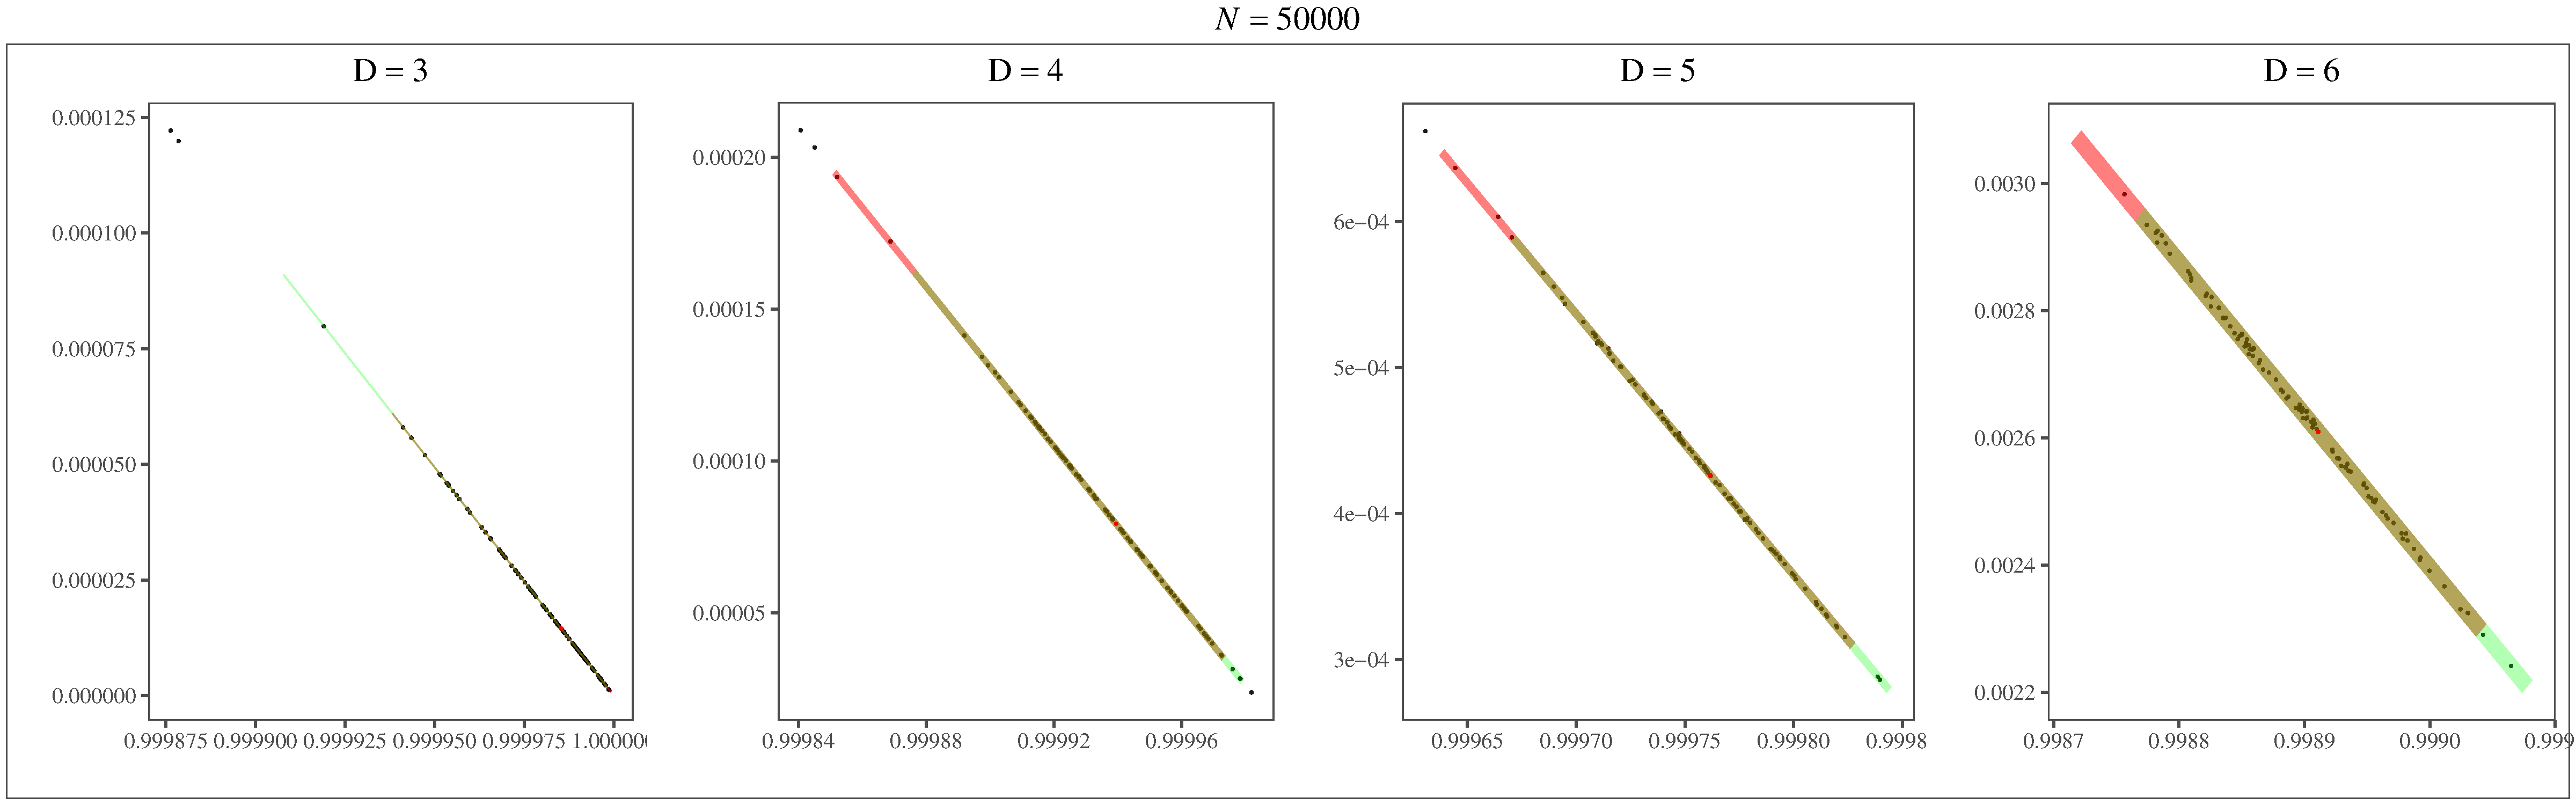
\includegraphics[width=\linewidth]{Figures/RNG-50000.pdf}
    \caption{Results of the analysis behavior of true random noises in the regions of confidence built.}
    \label{fig:RNG}
\end{figure}

\subsection{Analyzing Robustness to Correlation Structures}
% k=0 white
% k=1 pink
% k=2 brown
% T = 1000, T = 5 10^5
% D= 3, D = 6

Fig.~\ref{fig:AllSystems} shows the behavior of random time series with different levels of correlation (by means of the $f^{-k}$ model) in the $(h,c)$ plane.
Knowing that such plane can discriminate between different system dynamics, several studies in the literature have used this approach in the investigation of methods of identification and characterization of randomness.
Although this same strategy can be used to characterize different levels of correlation structures, in our case, we want to analyze the impact of injecting such dynamics into noise under the aspect of confidence regions.

For carrying out the experiment, we used an ''emblematic'' time series as a basis.
This series consists of the sample corresponding to the median of the $(h,c)$ points used to build the confidence regions, thus expressing a representative sample of the dataset.
Fig.~\ref{fig:correlation}a. illustrates, respectively, the effect of a white noise time series when adding correlation structures related to the $f^{-k}$ series for $k \in \{0, 1, 2, 3 \}$.
As we can observe in the plane as the correlation between the observations increases, that is, $k > 0$, the randomness decreases and the entropy presented decreases, informing the loss of its stochastic characteristic.

Fig.~\ref{fig:correlation}b. illustrates the degree of limit correlation structure that can be added in white noise to eliminate it from the regions of confidence, where the red dot represents the original "emblematic" series.
When we have $k = 0$, the features of the sequence have a small variation, corroborating the premise that series of noise $f^{-k} = 0$ have a minimum correlation measure, not significantly changing the dynamics of the system.

\begin{figure}
    \centering
	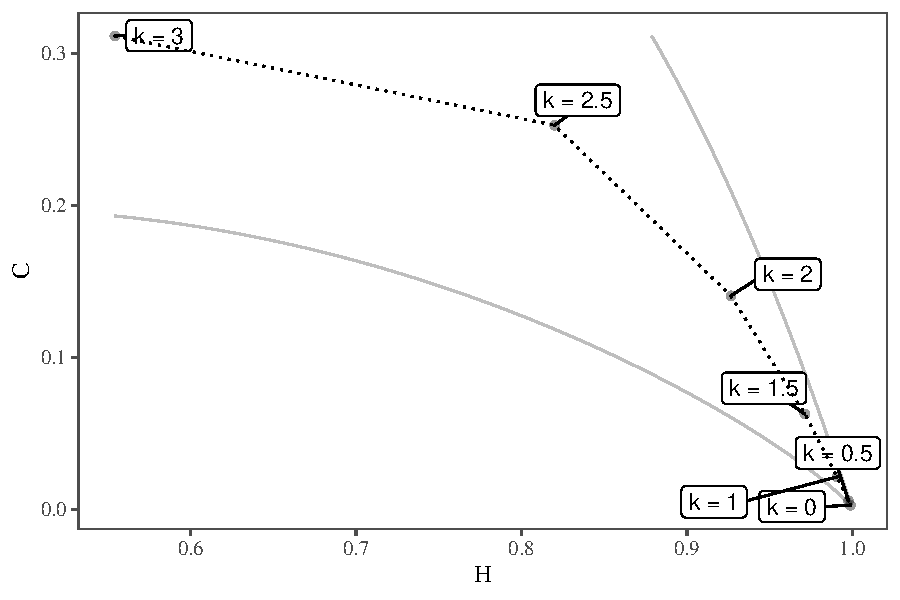
\includegraphics[width=.48\linewidth]{Figures/Correlation-Analysis-dotted.pdf}
    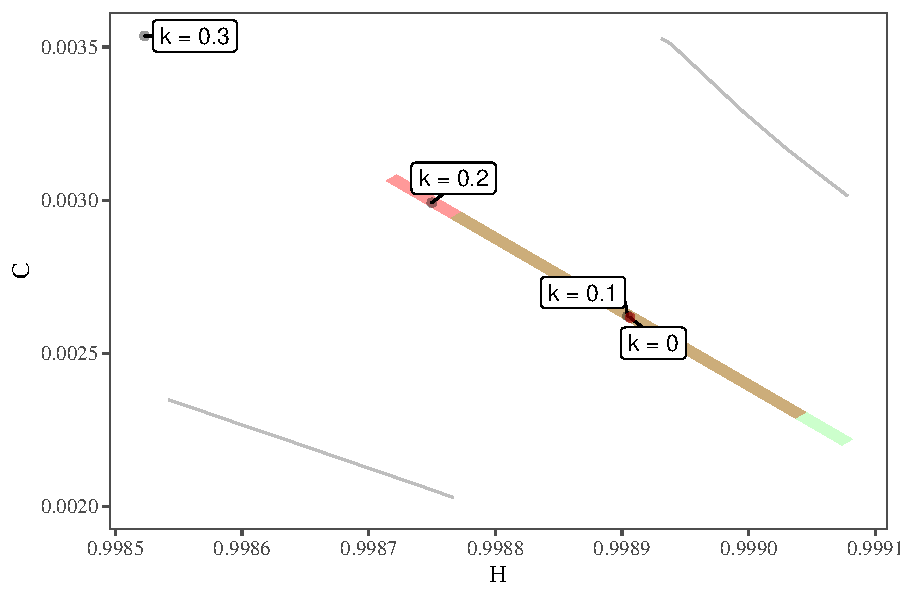
\includegraphics[width=.48\linewidth]{Figures/Correlation-Analysis-point.pdf}
    \caption{Correlation Structure Analysis}
    \label{fig:correlation}
\end{figure}

\subsection{Revisiting the White Noise Hypothesis in the Literature}

In this section, we evaluate the quality of the confidence regions preceded by HC-PCA with sequences of previously analyze generators in the literature with the Entropy-Complexity plane.
For this, we produced $100$ sequences of length $T = \num[scientific-notation=true]{5 e4}$ for each generator present in table~\ref{Tab:Literature} and calculated the respective p-values for each configuration of $D = \{3, 4, 5, 6\}$.
The results obtained can be seen in table~\ref{Tab:LiteratureComparations}, where we categorize the sets of sequences among those that did not reject (NR) the null hypothesis presented in the HC-PCA test and those that rejected (R).

Performing a comparative analysis of the results produced by tables~\ref{Tab:Literature} and~\ref{Tab:LiteratureComparations}, we can see that the proposed methodology of confidence regions can capture the random dynamics of the sequences produced by most of the analyzed generators well, although in our experiments we consider only short sequences.

However, two results deserve special attention: the sequences produced by the generators fBm and Combo RNG.
The first one, although it was not rejected by the analysis of~\cite{olivares2012contrasting}, presented low p-values, due to the characteristic point in the $H \times C$ plane where its sequences belong.
For the case analyzed in~\cite{olivares2012contrasting} with $D = 6$, we verified that the produced sequences present an average of $H = 0.997$, therefore they do not belong to the empirical $\SI{95}{\percent}$ confidence region produced by HC-PCA.
Analyzing the results produced by the Combo RNG, we can verify that only for $D = 3$ the proposed method can characterize the sequences produced as random.
This is due to the fact that by presenting higher dimension values, we were able to analyze a greater number of ordinal patterns, which may not be presented in their entirety in short sequences.

\begin{table}
    \caption{Results of the sequences generated by the main PRNGs in the literature. 
    The analyzed sequences have length $T=\num[scientific-notation = true]{5 e4}$.}
    \label{Tab:LiteratureComparations}
    \centering
    \begin{tabular}{cccc}
    \toprule
		Algorithm & 
		\multicolumn{1}{c}{$D$} & 
		$p$-value &
		HC-PCA\\
		\cmidrule(lr){1-1}
		\cmidrule(lr){2-2}
		\cmidrule(lr){3-3}
		\cmidrule(lr){4-4}
        MOT & 3 & 0.305 & NR\\
		& 4 & 0.572 & NR\\ 
		& 5 & 0.455 & NR\\ 
		& 6 & 0.508 & NR\\ 
		\cmidrule(lr){1-4}
        MWC & 3 & 0.501 & NR\\
        & 4 & 0.477 & NR\\ 
        & 5 & 0.496 & NR\\ 
        & 6 & 0.496 & NR\\ 
		\cmidrule(lr){1-4}
		COM & 3 & 0.123 & NR\\
		& 4 & 0.002 & R\\ 
		& 5 & \num[scientific-notation=true]{1.11 e-16} & R\\ 
		& 6 & \num[scientific-notation=true]{1.11 e-16} & R\\ 
		\cmidrule(lr){1-4}
		LEH & 3 & 0.531 & NR\\
		& 4 & 0.515 & NR\\ 
		& 5 & 0.495 & NR\\ 
		& 6 & 0.501 & NR\\ 
    \bottomrule
    \end{tabular}
    \begin{tabular}{|cccc}
    \toprule
		Algorithm & 
		\multicolumn{1}{c}{$D$} & 
		$p$-value &
		HC-PCA\\
		\cmidrule(lr){1-1}
		\cmidrule(lr){2-2}
		\cmidrule(lr){3-3}
		\cmidrule(lr){4-4}
		fGn & 3 & 0.521 & NR\\
		& 4 & 0.519 & NR\\ 
		& 5 & 0.498 & NR\\ 
		& 6 & 0.470 & NR\\
		\cmidrule(lr){1-4}
		fBm & 3 & \num[scientific-notation=true]{1.11 e-16} & R\\ 
		& 4 & \num[scientific-notation=true]{1.11 e-16} & R\\ 
		& 5 & \num[scientific-notation=true]{1.11 e-16} & R\\ 
		& 6 & \num[scientific-notation=true]{1.11 e-16} & R\\ 
		\cmidrule(lr){1-4}
		$f^{-k}$ & 3 & 0.482 & NR\\
		& 4 & 0.520 & NR\\ 
		& 5 & 0.513 & NR\\ 
		& 6 & 0.508 & NR\\
		\cmidrule(lr){1-4}
		LCG & 3 & 0.009 & R\\ 
		& 4 & \num[scientific-notation=true]{1.11 e-16} & R\\ 
		& 5 & \num[scientific-notation=true]{1.11 e-16} & R\\ 
		& 6 & \num[scientific-notation=true]{1.11 e-16} & R\\ 
    \bottomrule
    \end{tabular}
\end{table}

\begin{comment}
\begin{table}
    \caption{Results of literature PRNG references for time series of size $T = 50000$}
    \label{Tab:LiteratureComparations}
    \centering
    \begin{tabular}{c*{3}rcccc}
    \toprule
		Algorithm & 
		\multicolumn{1}{c}{$D$} & \multicolumn{1}{c}{\SI{95}{\percent}} & \multicolumn{1}{c}{\SI{99}{\percent}} & 
		$p$-value &
		HC-PCA & 
		Literature Results & 
		TestU01\\
		\cmidrule(lr){1-1}
		\cmidrule(lr){2-2}
		\cmidrule(lr){3-3}
		\cmidrule(lr){4-4}
		\cmidrule(lr){5-5}
		\cmidrule(lr){6-6}
		\cmidrule(lr){7-7}
		\cmidrule(lr){8-8}
        MOT & 3 & 1 & 1 & 0.305 & NR & NR & \\
		& 4 & 1 & 1 & 0.572  & & & \\ 
		& 5 & 1 & 1 & 0.455 & & & \\ 
		& 6 & 0.75 & 1 & 0.508 & & & \\ 
		\cmidrule(lr){1-8}
        MWC & 3 & 0.97 & 0.9625 & 0.501  & NR & NR & R\\
        & 4 & 0.97 & 0.9825 & 0.477 & & & \\ 
        & 5 & 0.9625 & 0.9625 & 0.496 & & & \\ 
        & 6 & 0.9675 & 0.9625 & 0.496  & & & \\ 
		\cmidrule(lr){1-8}
		COM & 3 & 0.25 & 0.5 & 0.123 & NR & NR & \\
		& 4 & 0 & 0 & 0.002 & R & & \\ 
		& 5 & 0 & 0 & \num[scientific-notation=true]{1.11 e-16} & & & \\ 
		& 6 & 0 & 0 & \num[scientific-notation=true]{1.11 e-16}  & & & \\ 
		\cmidrule(lr){1-8}
		LEH & 3 & 0.9825 & 0.98 & 0.531 & NR & NR & NR\\
		& 4 & 0.9675 & 0.9775 &  0.515  & & & \\ 
		& 5 & 0.9725 & 0.9775 &  0.495 & & & \\ 
		& 6 & 0.9775 & 0.9825 & 0.501 & & & \\ 
		\cmidrule(lr){1-8}
		fGn & 3 & 0.9722 & 0.9874 & 0.521 & NR & NR & \\
		& 4 & 0.9798 & 0.9773 & 0.519 & & & \\ 
		& 5 & 0.9646 & 0.9773 & 0.498 & & & \\ 
		& 6 & 0.9722 & 0.9545 & 0.470 & & & \\
		\cmidrule(lr){1-8}
		fBm & 3 & 0 & 0 & \num[scientific-notation=true]{1.11 e-16} & R & NR & \\ 
		& 4 & 0 & 0 & \num[scientific-notation=true]{1.11 e-16} & & & \\ 
		& 5 & 0 & 0 & \num[scientific-notation=true]{1.11 e-16} & & & \\ 
		& 6 & 0 & 0 & \num[scientific-notation=true]{1.11 e-16} & & & \\ 
		\cmidrule(lr){1-8}
		$f^{-k}$ & 3 & 0.9525 & 0.96 & 0.482 & NR & NR &\\
		& 4 & 0.975 & 0.9725 & 0.520 & & & \\ 
		& 5 & 0.98 & 0.9675 & 0.513 & & & \\ 
		& 6 & 0.9775 & 0.975 & 0.508 & & & \\
		\cmidrule(lr){1-8}
		LCG & 3 & 0.07 & 0.09 & 0.009 & R & R & R \\ 
		& 4 & 0 & 0 & \num[scientific-notation=true]{1.11 e-16} & & & \\ 
		& 5 & 0 & 0 & \num[scientific-notation=true]{1.11 e-16} & & & \\ 
		& 6 & 0 & 0 & \num[scientific-notation=true]{1.11 e-16} & & & \\ 
    \bottomrule
    \end{tabular}
\end{table}
\end{comment}

\begin{comment}
\begin{table}
	\centering
	\caption{Results of analysis of PRNGs with the proposed methodology}
	\label{tab:resultFinal}
	\begin{tabular}{c*{3}rccc}
		\toprule
		Algorithm & 
		\multicolumn{1}{c}{$D$} & 
		\multicolumn{1}{c}{\SI{95}{\percent}} & \multicolumn{1}{c}{\SI{99}{\percent}} &  
		$p$-value &
		HC-PCA &   
		TestU01\\
		\cmidrule(lr){1-1}
		\cmidrule(lr){2-2}
		\cmidrule(lr){3-3}
		\cmidrule(lr){4-4}
		\cmidrule(lr){5-5}
		\cmidrule(lr){6-6}
		\cmidrule(lr){7-7}
		Wichmann-Hill & 3 & 0.97 & 0.96 & 0.478 & NR & R\\ 
		& 4 & 0.9675 & 0.9675 & 0.513 & & \\ 
		& 5 & 0.9725 & 0.965 & 0.501 & & \\ 
		& 6 & 0.97 & 0.97 & 0.491 & & \\ 
		\cmidrule(lr){1-7}
		Super-Duper & 3 & 0.9675 & 0.975 & 0.496 & NR & R\\
		& 4 & 0.9775 & 0.9725 & 0.512 & &\\ 
		& 5 & 0.9675 & 0.985 & 0.525 & &\\ 
		& 6 & 0.9825 & 0.965 & 0.507 & &\\ 
		\cmidrule(lr){1-7}
		Knuth-TAOCP-2002 & 3 & 0.9775 & 0.9625 & 0.513 & NR & NR\\ 
		& 4 & 0.965 & 0.98 & 0.481 & &\\ 
		& 5 & 0.9625 & 0.9825 & 0.494 & &\\ 
		& 6 & 0.9725 & 0.96 & 0.479 & &\\  
		\cmidrule(lr){1-7}
		Knuth-TAOCP & 3 & 0.975 & 0.9775 & 0.480 & NR & NR\\
		& 4 & 0.965 & 0.9725 & 0.519 & &\\ 
		& 5 & 0.9875 & 0.985 & 0.531 & &\\ 
		& 6 & 0.9725 & 0.975 & 0.515 & &\\ 
		\cmidrule(lr){1-7}
		LEcuyer-CMRG & 3 & 0.98 & 0.98 & 0.505 & NR & NR\\ 
		& 4 & 0.9675 & 0.9725 & 0.490 & &\\ 
		& 5 & 0.965 & 0.9725 & 0.512 & &\\ 
		& 6 & 0.9625 & 0.97 & 0.524 & &\\ 
		\cmidrule(lr){1-7}
		Mersenne-Twister & 3 & 0.9725 & 0.97 & 0.506 & NR & NR\\ 
		& 4 & 0.98 & 0.97 & 0.499 & &\\ 
		& 5 & 0.9725 & 0.9775 & 0.524 & &\\ 
		& 6 & 0.975 & 0.9725 & 0.502 & &\\ 
		\cmidrule(lr){1-7}
		Randu & 3 & 0.2275 & 0.42 & 0.032 & R & R\\ 
		& 4 & 0 & 0 & \num[scientific-notation=true]{1.11 e-16} & &\\ 
		& 5 & 0 & 0 & \num[scientific-notation=true]{1.11 e-16} & &\\ 
		& 6 & 0 & 0 & \num[scientific-notation=true]{1.11 e-16} & &\\  
		\cmidrule(lr){1-7}
		pcg64 & 3 & 0.97 & 0.9675 & 0.510 & NR & NR\\
		& 4 & 0.97 & 0.97 & 0.503 & &\\ 
		& 5 & 0.9775 & 0.9625 & 0.508 & &\\ 
		& 6 & 0.9575 & 0.9575 & 0.502 & &\\ 
		\cmidrule(lr){1-7}
		Threefry & 3 & 0.9625 & 0.97 & 0.491 & NR & NR\\ 
		& 4 & 0.975 & 0.97 & 0.506 & &\\ 
		& 5 & 0.96 & 0.9625 & 0.506 & &\\ 
		& 6 & 0.965 & 0.955 & 0.473 & &\\ 
		\cmidrule(lr){1-7}
		Xoroshiro128+ & 3 & 0.975 & 0.9825 & 0.501 & NR & R\\ 
		& 4 & 0.995 & 0.9825 & 0.493 & &\\ 
		& 5 & 0.98 & 0.9725 & 0.503 & &\\ 
		& 6 & 0.9725 & 0.955 & 0.513 & &\\
		\cmidrule(lr){1-7}
		Xoshiro256+ & 3 & 0.98 & 0.98 & 0.502 & NR & NR\\ 
		& 4 & 0.9675 & 0.965 & 0.489 & &\\ 
		& 5 & 0.9525 & 0.96 & 0.492 & &\\ 
		& 6 & 0.9775 & 0.975 & 0.513 & &\\
		\bottomrule
	\end{tabular}
\end{table}
\end{comment}